
%%% Local Variables:
%%% mode: latex
%%% TeX-master: "chapter01"
%%% End:

\appendix
\renewcommand{\chaformat}[1]{%
    \parbox[b]{.8\textwidth}{\raggedleft\bfseries \S 附录 \\ \vspace{0.2ex} #1} \quad\rule[-12pt]{2pt}{70pt}\quad
    {\fontsize{60}{60}\selectfont\thechapter}}

\chapter{数据挖掘系统运行环境} \label{chpt:附录A}
数据挖掘系统运行环境包括数据挖掘系统主机、数据库系统主机和操作终端
三部分组成(见图\ref{fig:数据挖掘系统运行环境})。

\begin{figure}[!ht]
  \centering
  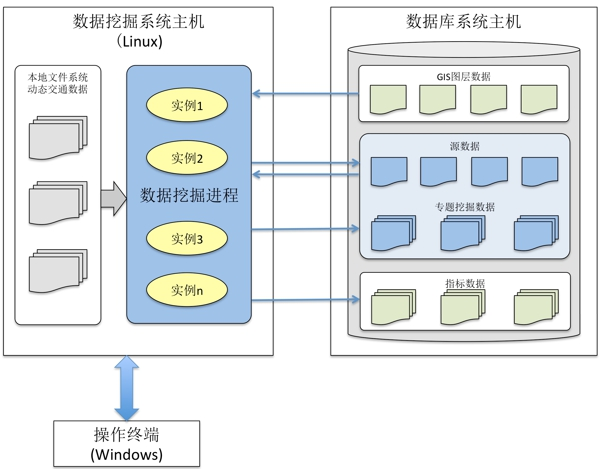
\includegraphics[width=0.8\textwidth]{数据挖掘系统运行环境.jpg}
  \caption{数据挖掘系统运行环境\label{fig:数据挖掘系统运行环境} }
\end{figure}


在深圳市交通仿真系统( 二期) 的设计中,数据挖掘系统主机主要负责对数
据进行挖掘运算,要求性能比较高,而且要求能够对待挖掘计算的原始数据进行
存储;数据库系统主机安装 Oracle 数据库, 负责存储挖掘计算之后的中间成果
数据库, 以及部分原始数据; 操作终端负责编写批处理指令,向数据挖掘系统主
机发送挖掘指令,远程控制整个挖掘计算的流程,并且能够对挖掘过程进行监控。三部分具体的配置情况见下表。

\renewcommand{\arraystretch}{0.8}
\begin{longtable}[c] {|C{0.15\textwidth}|C{0.25\textwidth}|C{0.25\textwidth}|C{0.2\textwidth}|}
  \caption{数据挖掘系统计算机环境配置\label{tbl:数据挖掘系统计算机环境配置}}
  \hline
  & \multicolumn{1}{c|}{\bfseries 数据挖掘系统主机} & \multicolumn{1}{c|}{\bfseries 数据库系统主机} &
  \multicolumn{1}{c|}{\bfseries 操作终端} \\\hline 

  IP 地址 & 192.168.114.123 & 192.168.114.111 & \\\hline
  操作系统 & CentOS 6.5 64 位 & CentOS 6.5 64 位 & Windows 7 \\\hline
  必备软件 & JDK 1.6 以上 & Oracle 11g & SecureCRT,FileZilla \\\hline
  登录信息 & 登录用户 dm,密码由管理员统一保管 & 登录用户 oracle; 数据库实例 JTFZ, 用户名 dm。 密码
由管理员统一保管 & 客户机自行设置 \\\hline
\end{longtable}

\chapter{数据查询系统运行环境} \label{chpt:附录B}
数据查询系统是一个标准的 B/S 三层结构设计,包括后台数据服务器主机、
web 应用服务器主机和前端操作终端主机三部分。

其中, 后台数据服务器主机负责存储指标数据库; web 应用服务器主机负责
为客户端的 HTTP 请求提供服务响应; 前端操作终端主机面向用户,由用户在浏
览器中通过点击、拖拽等操作向 web 应用服务器发送各种服务请求,并且将返
回的结果呈现在浏览器界面中。

按照深圳市交通仿真系统( 二期) 的设计, 三部分的具体配置情况见下表。

\renewcommand{\arraystretch}{0.8}
\begin{longtable}[c] {|C{0.12\textwidth}|C{0.25\textwidth}|C{0.3\textwidth}|C{0.2\textwidth}|}
  \caption{数据查询系统计算机环境配置\label{tbl:数据查询系统计算机环境配置}}
  \hline
  & \multicolumn{1}{c|}{\bfseries 数据服务器主机} & \multicolumn{1}{c|}{\bfseries web 应用服务器主机} &
  \multicolumn{1}{c|}{\bfseries 前端操作终端主机} \\\hline 

  IP 地址 & 192.168.114.111 & 192.168.114.101 & \\\hline
  操作系统 & CentOS 6.5 64 位 & Windows server 2008 & Windows 7 \\\hline
  必备软件 & Oracle 11g & Weblogic、ArcSDE 10.1、ArcGIS server 10.1、JDK 1.6 以上 & Flashplayer 11 以上;IE 7.0 以上, Chrome等主流浏览器 \\\hline
  登录信息 & 登录用户 oracle;数据库用户 szyw和 szjt,实例 JTFZ;密码由管理员统一保管 & 登录用户 administrator;
weblogic 用户 weblogic;ArcGIS server 用户 mono;密码由管理员保管 & 客户机自行设置\\\hline
\end{longtable}